\documentclass[twoside]{homework}
\usepackage{graphicx}

\studname{Geraldi Dzakwan (gd2551). Collaborators: None}
\studmail{gd2551@columbia.edu}
\coursename{COMS W4771: Machine Learning (sec:001)}
\hwNo{1}

\begin{document}
\maketitle

\section*{Problem 1}

\section*{Problem 2}

\begin{itemize}
    \item [(a)] Describe the algo
    \item [(b)] For $n=[1000, 2000, 4000, 8000]$, this is what I get:
        \begin{itemize}
            \item[]
            \begin{figure}[h!]
                \centering
                \includegraphics[scale=1]{nn_learning_curve}
                \caption{Nearest Neighbor Learning Curve}
                \label{fig:universe}
            \end{figure}
            \item[]
            \begin{table}[h!]
                \centering
                \begin{tabular}{||c c c||} 
                    \hline
                    $train\_size$ & $mean\_error$ & $std$ \\ [0.5ex] 
                    \hline\hline
                    1000 & 11.4850\% & 0.2984x$10^{-2}$ \\ 
                    \hline
                    2000 & 9.0010\% & 0.3022x$10^{-2}$ \\
                    \hline
                    4000 & 6.8820\% & 0.2098x$10^{-2}$ \\
                    \hline
                    8000 & 5.5780\% & 0.2041x$10^{-2}$ \\ [1ex] 
                    \hline
                \end{tabular}
                \caption{Nearest Neighbor Mean Error and Standard Deviation}
                \label{table:1}
            \end{table} 
        \end{itemize}
    \item [(c)] To do the 10-fold cross validation, I use Python \boldsymbol{sklearn} library. All training data are used, meaning that for each fold, 54000 data are for training and the remaining 6000 are for validation. This table below shows the cross validation error rate for each k.
        \begin{itemize}
            \begin{table}[h!]
                \centering
                \begin{tabular}{||c c||} 
                    \hline
                    $k$ & $cv\_error\_rate$ \\ [0.5ex] 
                    \hline\hline
                    1 & 2.9500\% \\ 
                    \hline
                    2 & 2.9500\% \\
                    \hline
                    \boldsymbol{3} & \boldsymbol{2.8233\%} \\
                    \hline
                    4 & 2.8700\% \\
                    \hline
                    5 & 2.9283\% \\
                    \hline
                    6 & 2.9533\% \\
                    \hline
                    7 & 3.0617\% \\
                    \hline
                    8 & 3.1200\% \\
                    \hline
                    9 & 3.2300\% \\
                    \hline
                    10 & 3.2633\% \\ [1ex] 
                    \hline
                \end{tabular}
                \caption{kNN Cross Validation Error Rates}
                \label{table:1}
            \end{table} 
        \end{itemize}
    From the table, we can see the optimal hyperparameter is \boldsymbol{k=3}. Using that value, I use full training data (60000 instances) and get test error rate (tested against 10000 data) of \boldsymbol{2.88\%}.
\end{itemize}

\section*{Problem 3}


\section*{Problem 4}
\begin{itemize}
    \item[(a)] We will consider these two ranges of x:
    \begin{itemize}
        \item[Case 1:] For $x\leq{0}$, $f_{\theta}(x)=0$. Thus, in this case, the likelihood is always zero and the MLE would be zero as well.
        \item[Case 2:]For $x>0$, $f_{\theta}(x)\propto{x^2}e^{-x/\theta}$. This means that $f_{\theta}(x)=c{x^2}e^{-x/\theta}$ for some constant c: $0<c<\infty$.
        Using the property that probability density functions should integrate to one, we can determine c:
        $$c\int_{0}^{\infty}{x^2}e^{-x/\theta}=1$$ 
        Using integration by parts, taking $u=x^2$ and $dv/dx=-{\theta}e^{-x/\theta}$, we get:
        $$-{\theta}e^{-x/\theta}x^2\Big|_0^{\infty}-\int_{0}^{\infty}(2x)(-{\theta}e^{-x/\theta})=1/c$$ 
        $$-{\theta}e^{-x/\theta}x^2\Big|_0^{\infty}+2\theta\int_{0}^{\infty}xe^{-x/\theta}=1/c$$ 
        Another integration by parts, taking $u=x$ and $dv/dx=-{\theta}e^{-x/\theta}$, we get:
        $$-{\theta}e^{-x/\theta}x^2\Big|_0^{\infty}+2\theta(-{\theta}e^{-x/\theta}x\Big|_0^{\infty}+\int_{0}^{\infty}{\theta}e^{-x\theta})=1/c$$
        $$-{\theta}e^{-x/\theta}x^2\Big|_0^{\infty}+2\theta(-{\theta}e^{-x/\theta}x\Big|_0^{\infty}-{\theta}^2e^{-x/\theta}\Big|_0^{\infty})=1/c$$ 
        $$-{\theta}e^{-x/\theta}x^2\Big|_0^{\infty}-2\theta^2e^{-x/\theta}x\Big|_0^{\infty}-2{\theta}^3e^{-x/\theta}\Big|_0^{\infty}=1/c$$ 
        $$-{\theta}e^{-x/\theta}x^2-2\theta^2e^{-x/\theta}x-2{\theta}^3e^{-x/\theta}\Big|_0^{\infty}=1/c$$ 
        \begin{itemize}
            \item[1.] Calculate upper bound:
            $$\text{upper\_bound}=-\theta\lim_{x\to\infty}\frac{x^2}{e^{x/\theta}}-2\theta^2\lim_{x\to\infty}\frac{x}{e^{x/\theta}}-2{\theta}^3\lim_{x\to\infty}\frac{1}{e^{x/\theta}}$$
            Using L'Hospital theorem a few times, we get:
            $$\text{upper\_bound}=-2\theta^2\lim_{x\to\infty}\frac{x}{e^{x/\theta}}-2\theta^3\lim_{x\to\infty}\frac{1}{e^{x/\theta}}-2\theta^3(0)$$
            $$\text{upper\_bound}=-2\theta^3\lim_{x\to\infty}\frac{1}{e^{x/\theta}}-2\theta^3(0)-2\theta^3(0)$$
            $$\text{upper\_bound}=-2\theta^3(0)-2\theta^3(0)-2\theta^3(0)=0$$
            \item[2.] Calculate lower bound:
            $$\text{lower\_bound}=-\theta\lim_{x\to{0}+}\frac{x^2}{e^{x/\theta}}-2\theta^2\lim_{x\to{0}+}\frac{x}{e^{x/\theta}}-2{\theta}^3\lim_{x\to{0}+}\frac{1}{e^{x/\theta}}$$
            $$\text{lower\_bound}=-\theta(\frac{0}{1})-2\theta^2(\frac{0}{1})-2{\theta}^3(\frac{1}{1})=-2{\theta}^3$$
        \end{itemize}
        Finally, $$\text{upper\_bound}-\text{lower\_bound}=1/c$$
        $$0-(-2\theta^3)=1/c$$
        $$c=1/(2\theta^3)$$
        Hence, the likelihood for $\{x_1,x_2,x_3,...,x_n\}$ would be:
        $$L(\theta|x)=\prod_{i=1}^{n} f_{\theta}(x_i) = (cx_i^2e^{-x_i/\theta})^n = (\frac{x_i^2e^{-x_i/\theta}}{2\theta^3})^n$$ 
        This is rather hard to expand, so we might want to take the log likelihood instead to determine the MLE:
        $$\ln{}L(\theta|x)=\ln(\prod_{i=1}^{n} f_{\theta}(x_i)) = \sum_{i=1}^n\ln(f_{\theta}(x_i)) = \sum_{i=1}^n\ln(\frac{x_i^2e^{-x_i/\theta}}{2\theta^3})$$
        $$\ln{}L(\theta|x)=\sum_{i=1}^n\ln{x_i^2}-\sum_{i=1}^n\ln{e^{x_i/\theta}}-\sum_{i=1}^n\ln{2\theta^3}$$
        $$\ln{}L(\theta|x)=2\sum_{i=1}^n\ln{x_i}-\sum_{i=1}^n(x_i/\theta)\ln{e}-\ln{2\theta^3}$$
        $$\ln{}L(\theta|x)=2\sum_{i=1}^n\ln{x_i}-\frac{1}{\theta}\sum_{i=1}^n{x_i}-\ln{2\theta^3}$$
        To minimize this, we can take its first derivative against $\theta$ and find the $\theta$ that makes it zero:
        $$\frac{d}{d\theta}\ln{}L(\theta|x) = 0$$
        $$0 + \frac{1}{\theta^2}\sum_{i=1}^n{x_i} - \frac{6\theta^2}{2\theta^3} = 0$$
        $$\frac{3}{\theta} = \frac{1}{\theta^2}\sum_{i=1}^n{x_i} \xrightarrow{} \theta = \frac{1}{3}\sum_{i=1}^n{x_i}$$
        Since $x>0$, this MLE formula will always be greater than zero, thus greater than MLE for case 1. Hence, we can pick this as our MLE formula.
    \end{itemize}
    $$\text{Thus, the MLE formula is }\boldsymbol{\hat{\theta}_{mle}=\frac{1}{3}\sum_{i=1}^n{x_i}}$$
    \item[(b)] We will consider these two ranges of x:
    \begin{itemize}
        \item[Case 1:] For $x<0$ and $x>\theta$, $f_{\theta}(x)=0$. Thus, in this case, the likelihood is always zero and the MLE would be zero as well.
        \item[Case 2:]For $0\leq{x}\leq{\theta}$, $f_{\theta}(x)\propto1$. This means that $f_{\theta}(x)=c$ for some constant c: $0<c<\infty$.
        Using the property that probability density functions should integrate to one, we can determine c:
        $$c\int_{0}^{\theta}dx=1$$ 
        $$cx\Big|_0^{\theta}=1$$ 
        $$c[\theta-0]=1$$
        $$c=1/\theta$$
        Hence, the likelihood for $\{x_1,x_2,x_3,...,x_n\}$ would be:
        $$L(\theta|x)=\prod_{i=1}^{n} f_{\theta}(x_i) = c^n = ({1/\theta})^n = 1/{\theta^n}$$
        To maximize that likelihood, we want to choose the smallest $\theta$ possible. Since we know that $0\leq{x}\leq{\theta}$, the smallest $\theta$ possible would be the the highest x in the set. Thus, the MLE formula would be:
        $\max(\{x_1, x_2, x_3, ..., x_n\})$. Since $0\leq{x}\leq{\theta}$ and $\theta>0$, this MLE formula will always be greater or equal to MLE for case 1 ($\geq{0})$. Hence, we can pick this as our MLE formula.
    \end{itemize}
    $$\text{Thus, the MLE formula is }\boldsymbol{\hat{\theta}_{mle}=\max(\{x_1, x_2, x_3, ..., x_n\})}$$
\end{itemize}

\section*{Problem 5}
\begin{itemize}
    \item[(a)] We can create a line of $x_1=2$ so that all the blue dots in the training data are on its right side, hence training false negative rate is zero. By drawing this line, there will be 3 false positives in the training data. Those are 3 red dots on the right side of the line. Thus, exactly $3/18=1/6$ training error. In this case, $\theta$ for $x_1$ will be 2, meanwhile for $x_2$ we don't need any $\theta$. This tree has depth equals to 1 (smallest) and can be coded as below.
                \begin{verbatim}
                    def d_tree_a(x1, x2):
                        if x1 < 2:
                            return 0
                        return 1
                \end{verbatim}
    \item[(b)] To make training rate equals to zero, we need to at least make a decision tree of depth 2. This is because there is no line $x_1=\theta_1$ or $x_2=\theta_2$ that can fully separate the red and blue dots. We can start with the previous value of $\theta_1=2$. Here, to make training rate equals to zero, we can pick any $\theta_2$ value between some value below 1 (probably around 0.6 by looking at the the picture) and some value below 2.2 (also by looking at the picture). \newline\newline
    To fulfill the second condition (test rate as high as possible), we need to look at the distribution of the test data. We can see that the test data distribution is almost the same as training data except that there are new blue dots in the range of $3<x_1<4$ and $1<x_2<2$. If we want to maximize test error, we should pick $\theta_2$ outside the range of $1<x_2<2$ so all the blue dots in that range will be classified as false negative. Thus, we can just pick $\theta_2=2$. This tree has depth equals to 2 (smallest) and can be coded as below.
                \begin{verbatim}
                    def d_tree_b(x1, x2):
                        if x1 < 2:
                            return 0
                        if x2 < 2:
                            return 0
                        return 1
                \end{verbatim}
\end{itemize}

\section*{Problem 6}
\begin{itemize}
    \item [(a)] Let X is random variable that denotes number of heads occurring in two coin tosses ($X=[0,1,2]$). Then, we can define two probabilities below:
    $$P(X=0)=P(tails).P(tails)=(1/2)(1/2)=1/4$$
    $$P(X\geq1)=1-P(X=0)=1-(1/2)(1/2)=3/4$$
    Using those probabilities, $Y_1=1$ occurs when a person that has property P ($\theta$) gets at least one head $P(X\geq1)$ or when a person that doesn't have property P ($1-\theta$) get no heads $P(X=0)$. Thus, $P(Y_1)=1$ is:
    $$P(Y_1=1)=P(X=0)(1-\theta) + P(X\geq1)\theta$$
    $$P(Y_1=1)=(1/4)(1-\theta) + (3/4)\theta$$
    $$P(Y_1=1)=(1/2)\theta + (1/4)$$
    \item [(b)] For $\{y_1, y_2, y_3, ..., y_n\}$, the likelihood would be: 
    $$\prod_{i=1}^{n}f_{\theta}(y_i)=\binom{n}{y_i}\prod_{i=1}^{n}P(y_i=1)^y_iP(y_i=0)=\frac{n!}{(n-y_i)!y_i!}P(y_i=1)(1-P(y_i=0))$$
    
\end{itemize}

\section*{Problem 7}


\end{document} 

To verify its functionality, I create a simple code to do cross validation on an array of size 10 and it works. 
    \begin{verbatim}
        from sklearn.model_selection import KFold

        X = np.zeros(10)
        kf = KFold(n_splits=10)
        for train, test in kf.split(X):
            print("%s %s" % (train, test))
    \end{verbatim}
    \begin{figure}[h!]
                \centering
                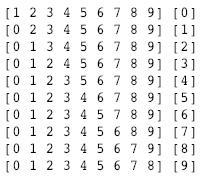
\includegraphics[scale=0.75]{verify_sklearn_cv.png}
                \caption{Verifying sklearn library cross validation}
                \label{fig:universe}
    \end{figure}
    
    $$\ln{L(\theta|x)}=n\ln{x^2}+n\ln{e^{-x/\theta}}-n\ln{2\theta^3}$$
        $$\ln{L(\theta|x)}=2n\ln{x}-(x/\theta)n\ln{e}-n\ln{2\theta^3}$$
        $$\ln{L(\theta|x)}=2n\ln{x}-(nx/\theta)-n\ln{2\theta^3}$$
